%%%%%%%%%%%%%%%%%%%%%%%%%%%%%%%%%%%%%%%%%
% Large Colored Title Article
% LaTeX Template
% Version 1.1 (25/11/12)
%
% This template has been downloaded from:
% http://www.LaTeXTemplates.com
%
% Original author:
% Frits Wenneker (http://www.howtotex.com)
%
% License:
% CC BY-NC-SA 3.0 (http://creativecommons.org/licenses/by-nc-sa/3.0/)
%
%%%%%%%%%%%%%%%%%%%%%%%%%%%%%%%%%%%%%%%%%

%----------------------------------------------------------------------------------------
%	PACKAGES AND OTHER DOCUMENT CONFIGURATIONS
%----------------------------------------------------------------------------------------

\documentclass[paper=a4, fontsize=11pt, onecolumn]{scrartcl}	 % A4 paper and 11pt font size

\usepackage{lipsum} % Used for inserting dummy 'Lorem ipsum' text into the template
\usepackage[english]{babel} % English language/hyphenation
\usepackage[protrusion=true,expansion=true]{microtype} % Better typography
\usepackage{amsmath,amsfonts,amsthm} % Math packages
\usepackage[svgnames]{xcolor} % Enabling colors by their 'svgnames'
\usepackage[hang, small,labelfont=bf,up,textfont=it,up]{caption} % Custom captions under/above floats in tables or figures
\usepackage{booktabs} % Horizontal rules in tables
\usepackage{fix-cm}	 % Custom font sizes - used for the initial letter in the document
\usepackage{graphicx}

\usepackage{sectsty} % Enables custom section titles
\allsectionsfont{\usefont{OT1}{phv}{b}{n}} % Change the font of all section commands

\usepackage{fancyhdr} % Needed to define custom headers/footers
\pagestyle{fancy} % Enables the custom headers/footers
\usepackage{lastpage} % Used to determine the number of pages in the document (for "Page X of Total")

% Headers - all currently empty
\lhead{}
\chead{}
\rhead{}

% Footers
\lfoot{}
\cfoot{}
\rfoot{\footnotesize Page \thepage\ of \pageref{LastPage}} % "Page 1 of 2"

\renewcommand{\headrulewidth}{0.0pt} % No header rule
\renewcommand{\footrulewidth}{0.4pt} % Thin footer rule

\usepackage{lettrine} % Package to accentuate the first letter of the text
\newcommand{\initial}[1]{ % Defines the command and style for the first letter
\lettrine[lines=3,lhang=0.3,nindent=0em]{
\color{DarkGoldenrod}
{\textsf{#1}}}{}}

%----------------------------------------------------------------------------------------
%	TITLE SECTION
%----------------------------------------------------------------------------------------

\usepackage{titling} % Allows custom title configuration

\newcommand{\HorRule}{\color{DarkGoldenrod} \rule{\linewidth}{1pt}} % Defines the gold horizontal rule around the title

\pretitle{\vspace{-30pt} \begin{flushleft} \HorRule \fontsize{50}{50} \usefont{OT1}{phv}{b}{n} \color{DarkRed} \selectfont} % Horizontal rule before the title

\title{FIR Filter} % Your article title

\posttitle{\par\end{flushleft}\vskip 0.5em} % Whitespace under the title

\preauthor{\begin{flushleft}\large \lineskip 0.5em \usefont{OT1}{phv}{b}{sl} \color{DarkRed}} % Author font configuration

\author{Ali Alipour Fraidani, } % Your name

\postauthor{\footnotesize \usefont{OT1}{phv}{m}{sl} \color{Black} % Configuration for the institution name
University of Tehran % Your institution

\par\end{flushleft}\HorRule} % Horizontal rule after the title

\date{} % Add a date here if you would like one to appear underneath the title block

%----------------------------------------------------------------------------------------

\begin{document}

\maketitle % Print the title

\thispagestyle{fancy} % Enabling the custom headers/footers for the first page 

%----------------------------------------------------------------------------------------
%	ABSTRACT
%----------------------------------------------------------------------------------------

% The first character should be within \initial{}
\initial{F}\textbf{inite Impulse Response (FIR) filters are a type of digital filter widely used in signal processing due to their simplicity, stability, and flexibility.}

%----------------------------------------------------------------------------------------
%	ARTICLE CONTENTS
%----------------------------------------------------------------------------------------

\section*{Key Characteristics of FIR Filters}

\begin{enumerate}
    \item \textbf{Finite Impulse Response:}
    \begin{itemize}
        \item The term ``finite impulse response'' indicates that the filter's impulse response settles to zero in a finite amount of time. This is because FIR filters do not have feedback loops, so the output is entirely based on a finite number of input samples.
    \end{itemize}

    \item \textbf{Linear Phase Response:}
    \begin{itemize}
        \item FIR filters can be designed to have a linear phase response, which means they preserve the phase relationships of the frequency components of the signal. This is important in applications like audio processing, where phase distortion is undesirable.
    \end{itemize}

    \item \textbf{Stability:}
    \begin{itemize}
        \item FIR filters are inherently stable because they lack feedback. The output depends only on current and past input values.
    \end{itemize}

    \item \textbf{Flexibility:}
    \begin{itemize}
        \item FIR filters can be designed to approximate almost any frequency response, making them suitable for a wide range of applications.
    \end{itemize}
\end{enumerate}

An FIR filter processes an input signal using the following equation:
\[
\text{What is the output } y[n] \text{ of the system defined as } 
y[n] = \sum_{k=0}^{N-1} h[k] \cdot x[n-k] \,
\]

\section*{Project explanation}

% \lipsum[1-3] % Dummy text

% \begin{align}
% A = 
% \begin{bmatrix}
% A_{11} & A_{21} \\
% A_{21} & A_{22}
% \end{bmatrix}
% \end{align}

As illustrated in Figure 1, the FIR filter has been implemented using a block diagram approach. In this design, the input and output bit widths are defined as parameters, enabling the designer to customize these values according to the required filter order. In this particular case, a 5th-order filter has been implemented. However, thanks to the parametric design, the filter order can be easily modified by adjusting the relevant parameters.

\begin{figure}[ht]
  \centering
  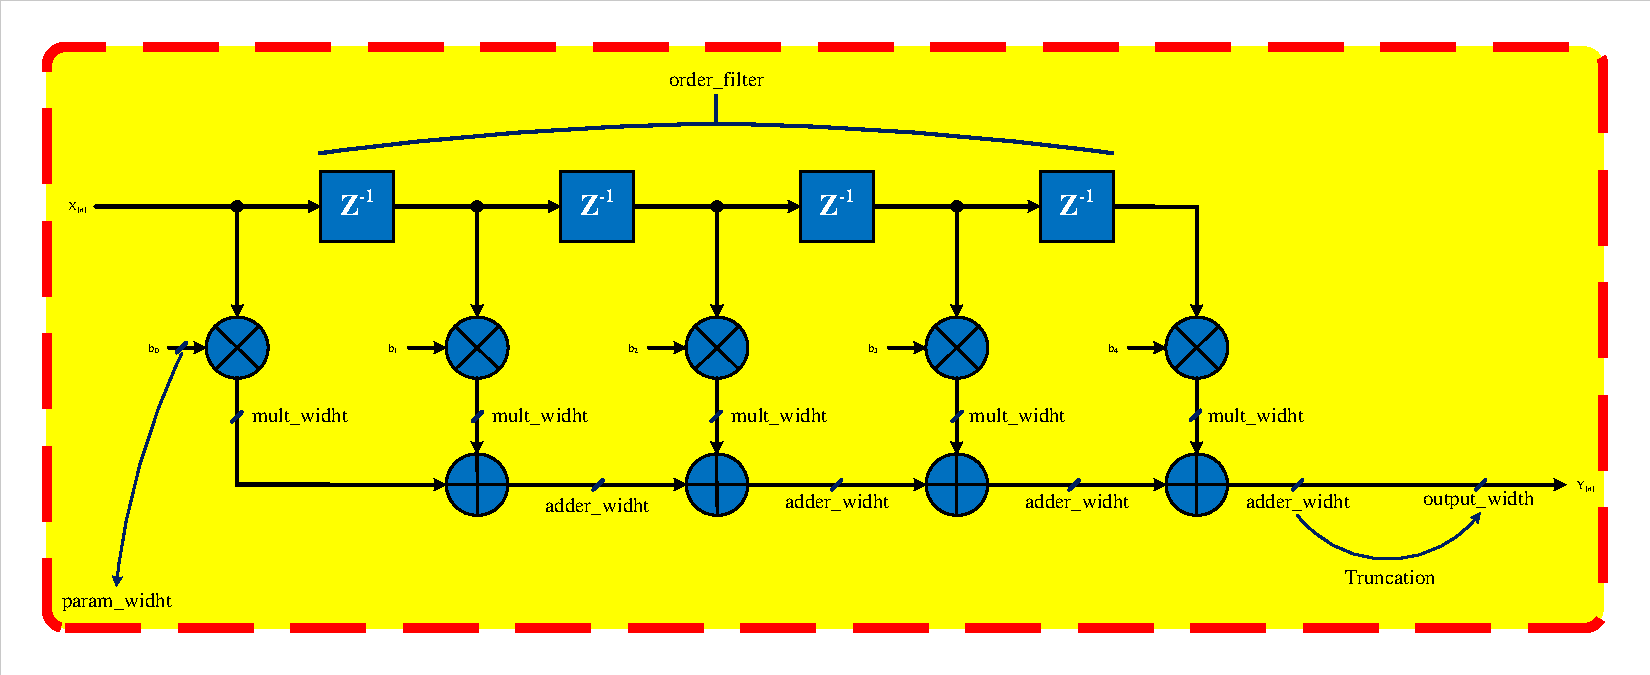
\includegraphics[width=0.5\textwidth]{FIR.pdf}
  \caption{FIR Filter}
  \label{fig:sample-image1}
\end{figure}

As shown in Figure 2, by utilizing this generated IP and modifying its parameters, the desired filter order can be adjusted as needed.

\begin{figure}[ht]
    \centering
    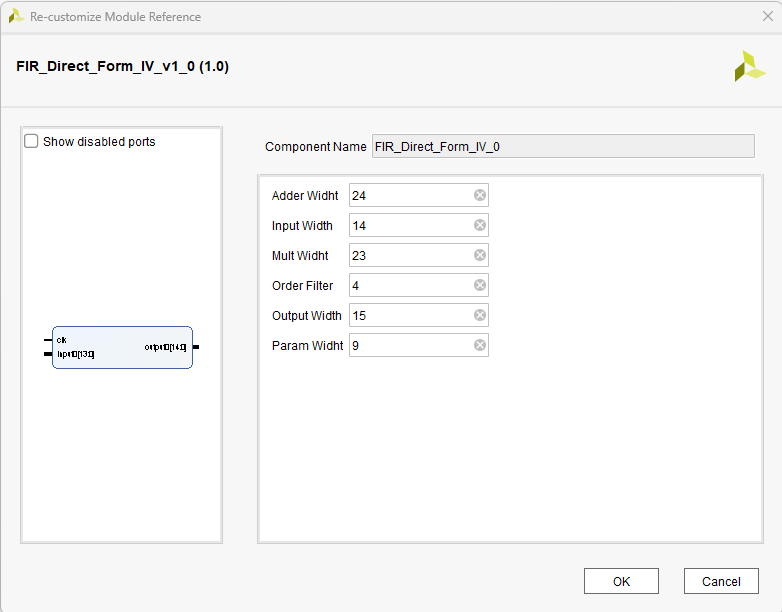
\includegraphics[width=0.5\textwidth]{"C:\\Users\\USER\\Documents\\Vivado_pro\\Session_2\\FIR Fileter\\Images\\Parameter_set.png"}
    \caption{IP Core}
    \label{fig:sample-image2}
\end{figure}

% \lipsum[4] % Dummy text

%------------------------------------------------

% \subsection*{Subsection 1}

% \lipsum[5] % Dummy text

% \begin{itemize}
% \item First item in a list 
% \item Second item in a list 
% \item Third item in a list
% \end{itemize}

% \lipsum[6] % Dummy text

%------------------------------------------------

% \subsection*{Subsection 2}

% \lipsum[7] % Dummy text

% \begin{table}
% \caption{Random table}
% \centering
% \begin{tabular}{llr}
% \toprule
% \multicolumn{2}{c}{Name} \\
% \cmidrule(r){1-2}
% First name & Last Name & Grade \\
% \midrule
% John & Doe & $7.5$ \\
% Richard & Miles & $2$ \\
% \bottomrule
% \end{tabular}
% \end{table}

% %------------------------------------------------

% \section*{Section 2}

% \lipsum[8] % Dummy text

% \begin{description}
% \item[First] This is the first item
% \item[Last] This is the last item
% \end{description}

% \lipsum[9] % Dummy text

%----------------------------------------------------------------------------------------
%	REFERENCE LIST
%----------------------------------------------------------------------------------------

% \begin{thebibliography}{99} % Bibliography - this is intentionally simple in this template

% \bibitem[Figueredo and Wolf, 2009]{Figueredo:2009dg}
% Figueredo, A.~J. and Wolf, P. S.~A. (2009).
% \newblock Assortative pairing and life history strategy - a cross-cultural
%   study.
% \newblock {\em Human Nature}, 20:317--330.
 
% \end{thebibliography}

%----------------------------------------------------------------------------------------

\end{document}